\normaltrue
\correctionfalse

%\UPSTIidClasse{11} % 11 sup, 12 spé
%\newcommand{\UPSTIidClasse}{12}

\exer{Mouvement RR  $\star$ \label{B2:13:04}}
\setcounter{numques}{0}
\UPSTIcompetence[2]{C2-05}
\UPSTIcompetence[2]{B2-13}
\index{Compétence C2-05}
\index{Compétence B2-13}
\index{Mécanisme à 2 rotations}
\ifcorrection
\else
\textbf{Pas de corrigé pour cet exercice.}
\fi

\ifprof
\else
Soit le mécanisme suivant. On a $\vect{AB}=R\vect{i_1}$ avec $R=\SI{20}{mm}$ et  
$\vect{BC}=L\vect{i_2}$ avec $L=\SI{15}{mm}$.
\begin{center}
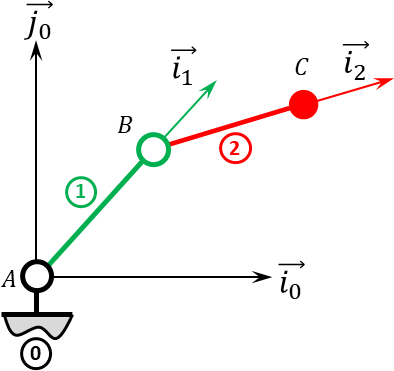
\includegraphics[width=\linewidth]{04_RR_01}
\end{center}
\fi

\question{Donner l'ensemble des positions accessibles par le point $C$.}
\ifprof~\\
Le point $C$ peut atteindre tous les points situés compris entre deux cercles de rayon \SI{5}{mm} et de rayon \SI{25}{mm}.
\else
\fi

\question{Donner l'équation du mouvement du point $C$ dans son mouvement de \textbf{2} par rapport à \textbf{0}.}
\ifprof~\\
On  a $\vect{AC}=R\vi{1}+L\vi{2}$. On projetant ce vecteur dans le repère $\rep{A}{i_0}{j_0}{k_0}$ on a 

$\vect{AC}=R\left(\cos\theta \vi{0} + \sin\theta \vj{0}\right) +L\left(\cos\left(\theta+\varphi\right) \vi{0} + \sin\left(\theta+\varphi\right) \vj{0}\right)$. On a donc :
$\left\{
\begin{array}{l}
x_C(t)= R\cos\theta  +L\cos\left(\theta+\varphi\right)  \\
y_C(t)= R \sin\theta + L\sin\left(\theta+\varphi\right)\\
z_C(t)= 0\\
\end{array}
\right.
$ dans le repère $\repere{A}{i_0}{j_0}{k_0}$.
\else
\fi

\ifprof
\else
On souhaite que le point $C$ réalise un segment entre les points $[-25,25]$ et $[25,25]$ à la vitesse linéaire $v$. 
\fi


\question{Donner la durée du mouvement si $C$ se déplace à vitesse quelconque.}
\ifprof ~\\
Distance à parcourir : $\SI{0,05}{m}$. Durée du parcours : $T=\dfrac{0,05}{v}$.
\else
\fi


\question{Donner l'équation paramétrique que doit suivre le point $C$.}
\ifprof ~\\
$\forall t \in \left[0,\dfrac{0,05}{v}\right]$, $y_C(t)=0,025$. 
Pour $t=0$, $x_C(0)=-0,025$. On a alors $x_C(t)=-0,025+vt$.  

Au final, $\forall t \in \left[0,\dfrac{0,05}{v}\right]$, $\left\{
\begin{array}{l}
x_C(t)= -0,025+vt\\
y_C(t)= 0,025\\
z_C(t)= 0\\
\end{array}
\right.
$ dans le repère $\repere{A}{i_0}{j_0}{k_0}$.


\else
\fi

\question{Donner les expressions de $\theta(t)$ et $\varphi(t)$ permettant la réalisation de cette trajectoire à la vitesse $v=\SI{0,01}{m.s^{-1}}$.}
\ifprof ~\\
Afin que le point $C$ suive un segment, il faut donc que 
$\left\{
\begin{array}{l}
-0,025+vt= R\cos\theta  +L\cos\left(\theta+\varphi\right)  \\
0,025 = R \sin\theta + L\sin\left(\theta+\varphi\right)\\
\end{array}
\right.
$

$\Leftrightarrow 
\left\{
\begin{array}{l}
-0,025+vt- R\cos\theta  =L\cos\left(\theta+\varphi\right)  \\
0,025 - R \sin\theta  = L\sin\left(\theta+\varphi\right)\\
\end{array}
\right.
$

$\Rightarrow 
\left\{
\begin{array}{l}
\left(-0,025+vt- R\cos\theta\right)^2  =L^2\cos^2\left(\theta+\varphi\right)  \\
\left(0,025 - R \sin\theta  \right)^2= L^2\sin^2\left(\theta+\varphi\right)\\
\end{array}
\right.
$

$\Rightarrow 
\left(-0,025+vt- R\cos\theta\right)^2  + \left(0,025 - R \sin\theta  \right)^2 = L^2
$

$\Rightarrow 
0,025^2+v^2t^2+R^2\cos^2\theta -2\times 0,025 vt+2R\cos\theta-vtR\cos\theta
  + 0,025^2 + R^2 \sin^2\theta -2\times 0,025 R \sin\theta  =      L^2
$

$\Rightarrow 
\left(2-vt\right)\cos\theta  -2\times 0,025  \sin\theta  =      \dfrac{L^2}{R} - \dfrac{2\times0,025^2}{R}-\dfrac{v^2t^2}{R}-R +2\times 0,025 \dfrac{vt}{R}
$


Équation trigonométrique de la forme $a\cos x  + b\sin x =c$.

Il y a donc une solution analytique. On peut aussi résoudre l'équation numériquement.


Une fois $\theta(t)$ déterminée, on a $0,025 - R \sin\theta  = L\sin\left(\theta+\varphi\right)$ 
$\Rightarrow \arcsin\left(\dfrac{0,025 - R \sin\theta(t)}{L}\right)  - \theta(t) = \varphi(t)$

\else
\fi


\question{En utilisant Python, tracer $\theta(t)$, $\varphi(t)$ et la trajectoire générée.}
\ifprof
\else
\fi


\ifprof
\else
\begin{flushright}
\footnotesize{Corrigé  voir \ref{B2:13:04}.}
\end{flushright}%
\fi